
        \documentclass[tikz, border=10pt]{standalone}
        \usepackage{tikz}
        \usetikzlibrary{arrows.meta, shapes, positioning}
        \usepackage{xcolor}
        \definecolor{brightmaroon}{RGB}{195,33,72}
\tikzset{bigbrightmaroonnode/.style={circle, fill=brightmaroon, draw=black, line width=1pt},
smallbrightmaroonnode/.style={circle, fill=brightmaroon, draw=black, line width=0.5pt, minimum size=4pt, inner sep=0pt}}
\definecolor{cyan}{RGB}{0,255,255}
\tikzset{bigcyannode/.style={circle, fill=cyan, draw=black, line width=1pt},
smallcyannode/.style={circle, fill=cyan, draw=black, line width=0.5pt, minimum size=4pt, inner sep=0pt}}
\definecolor{skyblue}{RGB}{135,206,235}
\tikzset{bigskybluenode/.style={circle, fill=skyblue, draw=black, line width=1pt},
smallskybluenode/.style={circle, fill=skyblue, draw=black, line width=0.5pt, minimum size=4pt, inner sep=0pt}}

        \begin{document}
            % Graph for 3 attributes
            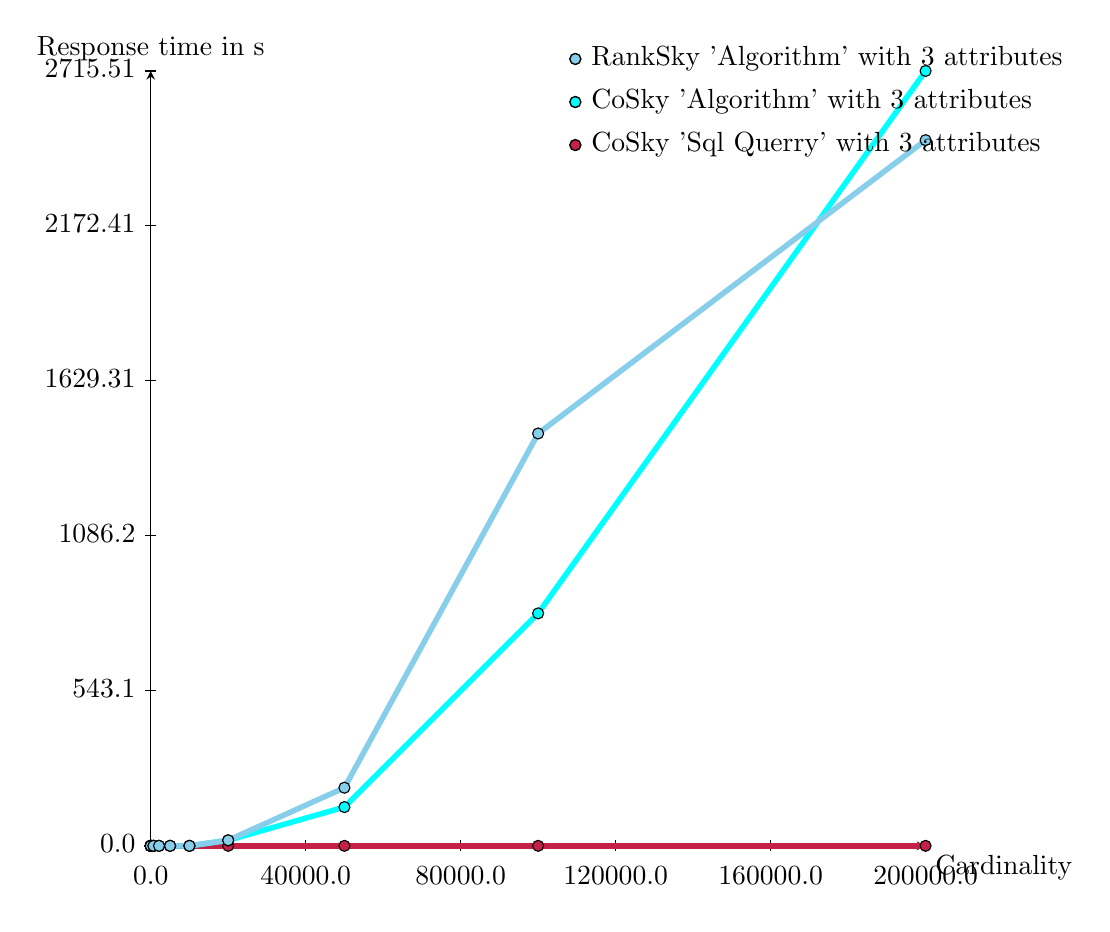
\begin{tikzpicture}[
                line join=bevel,
                smallbrightmaroonnode/.style={circle, fill=brightmaroon, draw=black, line width=0.5pt, minimum size=4pt, inner sep=0pt},
                smallcyannode/.style={circle, fill=cyan, draw=black, line width=0.5pt, minimum size=4pt, inner sep=0pt},
                smallskybluenode/.style={circle, fill=skyblue, draw=black, line width=0.5pt, minimum size=4pt, inner sep=0pt}
            ]
                \draw[-stealth] (0pt, 0pt) -- (280pt, 0pt) node[anchor=north west] {Cardinality};
                \draw[-stealth] (0pt, 0pt) -- (0pt, 280pt) node[anchor=south] {Response time in s};

                % Axis graduations
                \foreach \x/\xtext in {0pt/$0.0$, 56pt/$40000.0$, 112pt/$80000.0$, 168pt/$120000.0$, 224pt/$160000.0$, 280pt/$200000.0$} {
\draw (\x, 2pt) -- (\x, -2pt) node[below] {\xtext\strut};
}
                \foreach \y/\ytext in {0pt/$0.0$, 56pt/$543.1$, 112pt/$1086.2$, 168pt/$1629.31$, 224pt/$2172.41$, 280pt/$2715.51$} {
\draw (2pt, \y) -- (-2pt, \y) node[left] {\ytext\strut};
}

                % Curves
                \draw[brightmaroon, line width=2pt](0pt, 0pt) -- (0pt, 0pt) -- (0pt, 0pt) -- (0pt, 0pt) -- (0pt, 0pt) -- (1pt, 0pt) -- (1pt, 0pt) -- (3pt, 0pt) -- (7pt, 0pt) -- (14pt, 0pt) -- (28pt, 0pt) -- (70pt, 0pt) -- (140pt, 0pt) -- (280pt, 0pt);

                \draw[cyan, line width=2pt](0pt, 0pt) -- (0pt, 0pt) -- (0pt, 0pt) -- (0pt, 0pt) -- (0pt, 0pt) -- (1pt, 0pt) -- (1pt, 0pt) -- (3pt, 0pt) -- (7pt, 0pt) -- (14pt, 0pt) -- (28pt, 2pt) -- (70pt, 14pt) -- (140pt, 84pt) -- (280pt, 280pt);

                \draw[skyblue, line width=2pt](0pt, 0pt) -- (0pt, 0pt) -- (0pt, 0pt) -- (0pt, 0pt) -- (0pt, 0pt) -- (1pt, 0pt) -- (1pt, 0pt) -- (3pt, 0pt) -- (7pt, 0pt) -- (14pt, 0pt) -- (28pt, 2pt) -- (70pt, 21pt) -- (140pt, 149pt) -- (280pt, 255pt);


                % Points
                \filldraw[color=black, fill=brightmaroon] (0pt, 0pt) circle (2pt);
\filldraw[color=black, fill=brightmaroon] (0pt, 0pt) circle (2pt);
\filldraw[color=black, fill=brightmaroon] (0pt, 0pt) circle (2pt);
\filldraw[color=black, fill=brightmaroon] (0pt, 0pt) circle (2pt);
\filldraw[color=black, fill=brightmaroon] (0pt, 0pt) circle (2pt);
\filldraw[color=black, fill=brightmaroon] (1pt, 0pt) circle (2pt);
\filldraw[color=black, fill=brightmaroon] (1pt, 0pt) circle (2pt);
\filldraw[color=black, fill=brightmaroon] (3pt, 0pt) circle (2pt);
\filldraw[color=black, fill=brightmaroon] (7pt, 0pt) circle (2pt);
\filldraw[color=black, fill=brightmaroon] (14pt, 0pt) circle (2pt);
\filldraw[color=black, fill=brightmaroon] (28pt, 0pt) circle (2pt);
\filldraw[color=black, fill=brightmaroon] (70pt, 0pt) circle (2pt);
\filldraw[color=black, fill=brightmaroon] (140pt, 0pt) circle (2pt);
\filldraw[color=black, fill=brightmaroon] (280pt, 0pt) circle (2pt);

                \filldraw[color=black, fill=cyan] (0pt, 0pt) circle (2pt);
\filldraw[color=black, fill=cyan] (0pt, 0pt) circle (2pt);
\filldraw[color=black, fill=cyan] (0pt, 0pt) circle (2pt);
\filldraw[color=black, fill=cyan] (0pt, 0pt) circle (2pt);
\filldraw[color=black, fill=cyan] (0pt, 0pt) circle (2pt);
\filldraw[color=black, fill=cyan] (1pt, 0pt) circle (2pt);
\filldraw[color=black, fill=cyan] (1pt, 0pt) circle (2pt);
\filldraw[color=black, fill=cyan] (3pt, 0pt) circle (2pt);
\filldraw[color=black, fill=cyan] (7pt, 0pt) circle (2pt);
\filldraw[color=black, fill=cyan] (14pt, 0pt) circle (2pt);
\filldraw[color=black, fill=cyan] (28pt, 2pt) circle (2pt);
\filldraw[color=black, fill=cyan] (70pt, 14pt) circle (2pt);
\filldraw[color=black, fill=cyan] (140pt, 84pt) circle (2pt);
\filldraw[color=black, fill=cyan] (280pt, 280pt) circle (2pt);

                \filldraw[color=black, fill=skyblue] (0pt, 0pt) circle (2pt);
\filldraw[color=black, fill=skyblue] (0pt, 0pt) circle (2pt);
\filldraw[color=black, fill=skyblue] (0pt, 0pt) circle (2pt);
\filldraw[color=black, fill=skyblue] (0pt, 0pt) circle (2pt);
\filldraw[color=black, fill=skyblue] (0pt, 0pt) circle (2pt);
\filldraw[color=black, fill=skyblue] (1pt, 0pt) circle (2pt);
\filldraw[color=black, fill=skyblue] (1pt, 0pt) circle (2pt);
\filldraw[color=black, fill=skyblue] (3pt, 0pt) circle (2pt);
\filldraw[color=black, fill=skyblue] (7pt, 0pt) circle (2pt);
\filldraw[color=black, fill=skyblue] (14pt, 0pt) circle (2pt);
\filldraw[color=black, fill=skyblue] (28pt, 2pt) circle (2pt);
\filldraw[color=black, fill=skyblue] (70pt, 21pt) circle (2pt);
\filldraw[color=black, fill=skyblue] (140pt, 149pt) circle (2pt);
\filldraw[color=black, fill=skyblue] (280pt, 255pt) circle (2pt);


                % Caption
                \matrix [below left] at (current bounding box.north east) {
                    \node [smallskybluenode, label=right:RankSky 'Algorithm'  with 3 attributes] {}; \\
                    \node [smallcyannode, label=right:CoSky 'Algorithm'  with 3 attributes] {}; \\
                    \node [smallbrightmaroonnode, label=right:CoSky 'Sql Querry'  with 3 attributes] {}; \\
                };
            \end{tikzpicture}
            
            % Graph for 6 attributes
            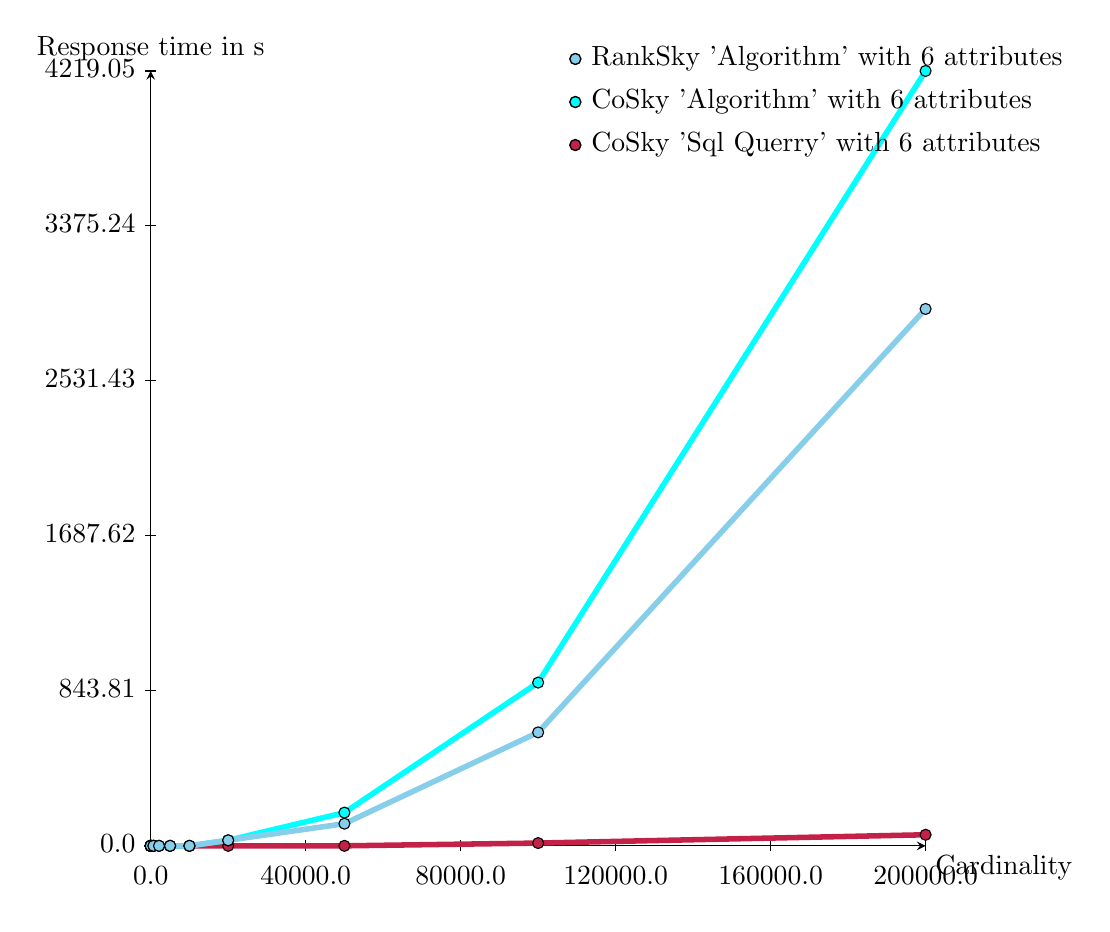
\begin{tikzpicture}[
                line join=bevel,
                smallbrightmaroonnode/.style={circle, fill=brightmaroon, draw=black, line width=0.5pt, minimum size=4pt, inner sep=0pt},
                smallcyannode/.style={circle, fill=cyan, draw=black, line width=0.5pt, minimum size=4pt, inner sep=0pt},
                smallskybluenode/.style={circle, fill=skyblue, draw=black, line width=0.5pt, minimum size=4pt, inner sep=0pt}
            ]
                \draw[-stealth] (0pt, 0pt) -- (280pt, 0pt) node[anchor=north west] {Cardinality};
                \draw[-stealth] (0pt, 0pt) -- (0pt, 280pt) node[anchor=south] {Response time in s};

                % Axis graduations
                \foreach \x/\xtext in {0pt/$0.0$, 56pt/$40000.0$, 112pt/$80000.0$, 168pt/$120000.0$, 224pt/$160000.0$, 280pt/$200000.0$} {
\draw (\x, 2pt) -- (\x, -2pt) node[below] {\xtext\strut};
}
                \foreach \y/\ytext in {0pt/$0.0$, 56pt/$843.81$, 112pt/$1687.62$, 168pt/$2531.43$, 224pt/$3375.24$, 280pt/$4219.05$} {
\draw (2pt, \y) -- (-2pt, \y) node[left] {\ytext\strut};
}

                % Curves
                \draw[brightmaroon, line width=2pt](0pt, 0pt) -- (0pt, 0pt) -- (0pt, 0pt) -- (0pt, 0pt) -- (0pt, 0pt) -- (1pt, 0pt) -- (1pt, 0pt) -- (3pt, 0pt) -- (7pt, 0pt) -- (14pt, 0pt) -- (28pt, 0pt) -- (70pt, 0pt) -- (140pt, 1pt) -- (280pt, 4pt);

                \draw[cyan, line width=2pt](0pt, 0pt) -- (0pt, 0pt) -- (0pt, 0pt) -- (0pt, 0pt) -- (0pt, 0pt) -- (1pt, 0pt) -- (1pt, 0pt) -- (3pt, 0pt) -- (7pt, 0pt) -- (14pt, 0pt) -- (28pt, 2pt) -- (70pt, 12pt) -- (140pt, 59pt) -- (280pt, 280pt);

                \draw[skyblue, line width=2pt](0pt, 0pt) -- (0pt, 0pt) -- (0pt, 0pt) -- (0pt, 0pt) -- (0pt, 0pt) -- (1pt, 0pt) -- (1pt, 0pt) -- (3pt, 0pt) -- (7pt, 0pt) -- (14pt, 0pt) -- (28pt, 2pt) -- (70pt, 8pt) -- (140pt, 41pt) -- (280pt, 194pt);


                % Points
                \filldraw[color=black, fill=brightmaroon] (0pt, 0pt) circle (2pt);
\filldraw[color=black, fill=brightmaroon] (0pt, 0pt) circle (2pt);
\filldraw[color=black, fill=brightmaroon] (0pt, 0pt) circle (2pt);
\filldraw[color=black, fill=brightmaroon] (0pt, 0pt) circle (2pt);
\filldraw[color=black, fill=brightmaroon] (0pt, 0pt) circle (2pt);
\filldraw[color=black, fill=brightmaroon] (1pt, 0pt) circle (2pt);
\filldraw[color=black, fill=brightmaroon] (1pt, 0pt) circle (2pt);
\filldraw[color=black, fill=brightmaroon] (3pt, 0pt) circle (2pt);
\filldraw[color=black, fill=brightmaroon] (7pt, 0pt) circle (2pt);
\filldraw[color=black, fill=brightmaroon] (14pt, 0pt) circle (2pt);
\filldraw[color=black, fill=brightmaroon] (28pt, 0pt) circle (2pt);
\filldraw[color=black, fill=brightmaroon] (70pt, 0pt) circle (2pt);
\filldraw[color=black, fill=brightmaroon] (140pt, 1pt) circle (2pt);
\filldraw[color=black, fill=brightmaroon] (280pt, 4pt) circle (2pt);

                \filldraw[color=black, fill=cyan] (0pt, 0pt) circle (2pt);
\filldraw[color=black, fill=cyan] (0pt, 0pt) circle (2pt);
\filldraw[color=black, fill=cyan] (0pt, 0pt) circle (2pt);
\filldraw[color=black, fill=cyan] (0pt, 0pt) circle (2pt);
\filldraw[color=black, fill=cyan] (0pt, 0pt) circle (2pt);
\filldraw[color=black, fill=cyan] (1pt, 0pt) circle (2pt);
\filldraw[color=black, fill=cyan] (1pt, 0pt) circle (2pt);
\filldraw[color=black, fill=cyan] (3pt, 0pt) circle (2pt);
\filldraw[color=black, fill=cyan] (7pt, 0pt) circle (2pt);
\filldraw[color=black, fill=cyan] (14pt, 0pt) circle (2pt);
\filldraw[color=black, fill=cyan] (28pt, 2pt) circle (2pt);
\filldraw[color=black, fill=cyan] (70pt, 12pt) circle (2pt);
\filldraw[color=black, fill=cyan] (140pt, 59pt) circle (2pt);
\filldraw[color=black, fill=cyan] (280pt, 280pt) circle (2pt);

                \filldraw[color=black, fill=skyblue] (0pt, 0pt) circle (2pt);
\filldraw[color=black, fill=skyblue] (0pt, 0pt) circle (2pt);
\filldraw[color=black, fill=skyblue] (0pt, 0pt) circle (2pt);
\filldraw[color=black, fill=skyblue] (0pt, 0pt) circle (2pt);
\filldraw[color=black, fill=skyblue] (0pt, 0pt) circle (2pt);
\filldraw[color=black, fill=skyblue] (1pt, 0pt) circle (2pt);
\filldraw[color=black, fill=skyblue] (1pt, 0pt) circle (2pt);
\filldraw[color=black, fill=skyblue] (3pt, 0pt) circle (2pt);
\filldraw[color=black, fill=skyblue] (7pt, 0pt) circle (2pt);
\filldraw[color=black, fill=skyblue] (14pt, 0pt) circle (2pt);
\filldraw[color=black, fill=skyblue] (28pt, 2pt) circle (2pt);
\filldraw[color=black, fill=skyblue] (70pt, 8pt) circle (2pt);
\filldraw[color=black, fill=skyblue] (140pt, 41pt) circle (2pt);
\filldraw[color=black, fill=skyblue] (280pt, 194pt) circle (2pt);


                % Caption
                \matrix [below left] at (current bounding box.north east) {
                    \node [smallskybluenode, label=right:RankSky 'Algorithm'  with 6 attributes] {}; \\
                    \node [smallcyannode, label=right:CoSky 'Algorithm'  with 6 attributes] {}; \\
                    \node [smallbrightmaroonnode, label=right:CoSky 'Sql Querry'  with 6 attributes] {}; \\
                };
            \end{tikzpicture}
            
            % Graph for 9 attributes
            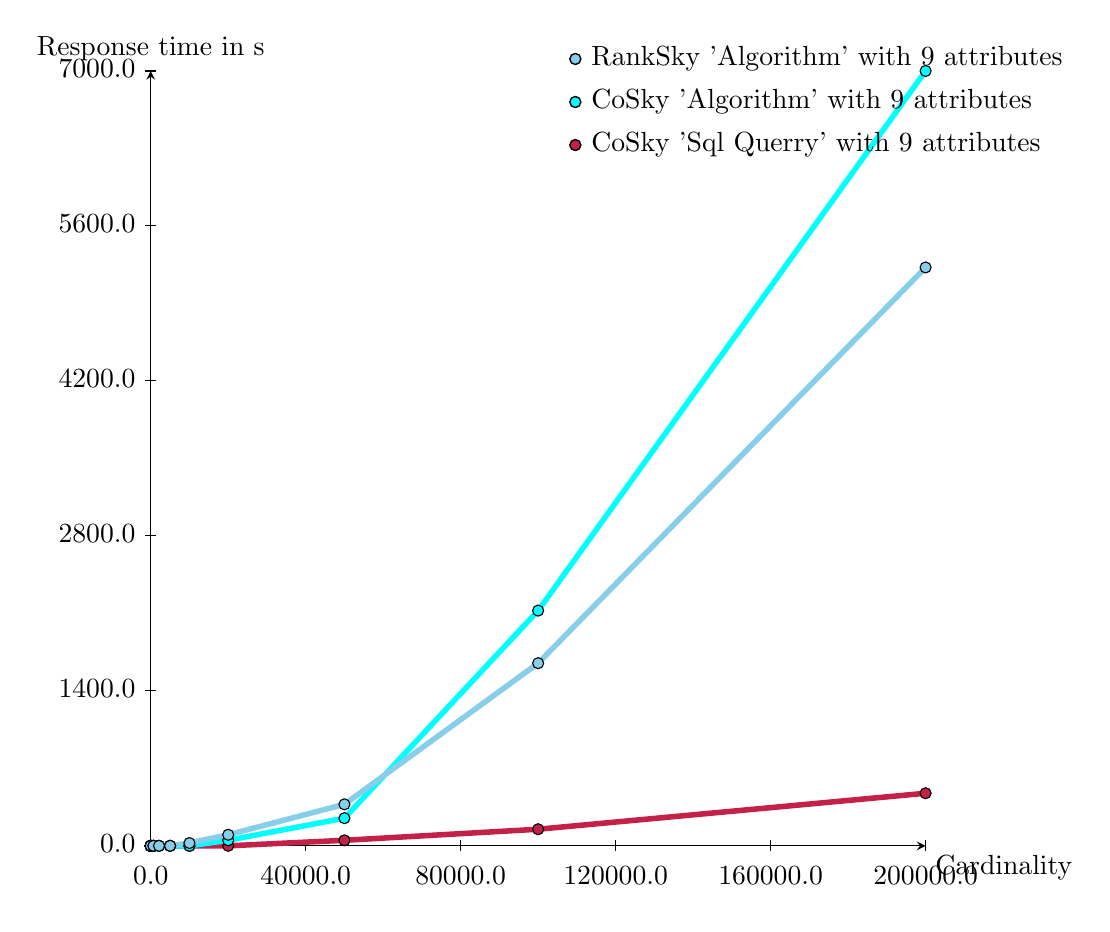
\begin{tikzpicture}[
                line join=bevel,
                smallbrightmaroonnode/.style={circle, fill=brightmaroon, draw=black, line width=0.5pt, minimum size=4pt, inner sep=0pt},
                smallcyannode/.style={circle, fill=cyan, draw=black, line width=0.5pt, minimum size=4pt, inner sep=0pt},
                smallskybluenode/.style={circle, fill=skyblue, draw=black, line width=0.5pt, minimum size=4pt, inner sep=0pt}
            ]
                \draw[-stealth] (0pt, 0pt) -- (280pt, 0pt) node[anchor=north west] {Cardinality};
                \draw[-stealth] (0pt, 0pt) -- (0pt, 280pt) node[anchor=south] {Response time in s};

                % Axis graduations
                \foreach \x/\xtext in {0pt/$0.0$, 56pt/$40000.0$, 112pt/$80000.0$, 168pt/$120000.0$, 224pt/$160000.0$, 280pt/$200000.0$} {
\draw (\x, 2pt) -- (\x, -2pt) node[below] {\xtext\strut};
}
                \foreach \y/\ytext in {0pt/$0.0$, 56pt/$1400.0$, 112pt/$2800.0$, 168pt/$4200.0$, 224pt/$5600.0$, 280pt/$7000.0$} {
\draw (2pt, \y) -- (-2pt, \y) node[left] {\ytext\strut};
}

                % Curves
                \draw[brightmaroon, line width=2pt](0pt, 0pt) -- (0pt, 0pt) -- (0pt, 0pt) -- (0pt, 0pt) -- (0pt, 0pt) -- (1pt, 0pt) -- (1pt, 0pt) -- (3pt, 0pt) -- (7pt, 0pt) -- (14pt, 0pt) -- (28pt, 0pt) -- (70pt, 2pt) -- (140pt, 6pt) -- (280pt, 19pt);

                \draw[cyan, line width=2pt](0pt, 0pt) -- (0pt, 0pt) -- (0pt, 0pt) -- (0pt, 0pt) -- (0pt, 0pt) -- (1pt, 0pt) -- (1pt, 0pt) -- (3pt, 0pt) -- (7pt, 0pt) -- (14pt, 0pt) -- (28pt, 2pt) -- (70pt, 10pt) -- (140pt, 85pt) -- (280pt, 280pt);

                \draw[skyblue, line width=2pt](0pt, 0pt) -- (0pt, 0pt) -- (0pt, 0pt) -- (0pt, 0pt) -- (0pt, 0pt) -- (1pt, 0pt) -- (1pt, 0pt) -- (3pt, 0pt) -- (7pt, 0pt) -- (14pt, 1pt) -- (28pt, 4pt) -- (70pt, 15pt) -- (140pt, 66pt) -- (280pt, 209pt);


                % Points
                \filldraw[color=black, fill=brightmaroon] (0pt, 0pt) circle (2pt);
\filldraw[color=black, fill=brightmaroon] (0pt, 0pt) circle (2pt);
\filldraw[color=black, fill=brightmaroon] (0pt, 0pt) circle (2pt);
\filldraw[color=black, fill=brightmaroon] (0pt, 0pt) circle (2pt);
\filldraw[color=black, fill=brightmaroon] (0pt, 0pt) circle (2pt);
\filldraw[color=black, fill=brightmaroon] (1pt, 0pt) circle (2pt);
\filldraw[color=black, fill=brightmaroon] (1pt, 0pt) circle (2pt);
\filldraw[color=black, fill=brightmaroon] (3pt, 0pt) circle (2pt);
\filldraw[color=black, fill=brightmaroon] (7pt, 0pt) circle (2pt);
\filldraw[color=black, fill=brightmaroon] (14pt, 0pt) circle (2pt);
\filldraw[color=black, fill=brightmaroon] (28pt, 0pt) circle (2pt);
\filldraw[color=black, fill=brightmaroon] (70pt, 2pt) circle (2pt);
\filldraw[color=black, fill=brightmaroon] (140pt, 6pt) circle (2pt);
\filldraw[color=black, fill=brightmaroon] (280pt, 19pt) circle (2pt);

                \filldraw[color=black, fill=cyan] (0pt, 0pt) circle (2pt);
\filldraw[color=black, fill=cyan] (0pt, 0pt) circle (2pt);
\filldraw[color=black, fill=cyan] (0pt, 0pt) circle (2pt);
\filldraw[color=black, fill=cyan] (0pt, 0pt) circle (2pt);
\filldraw[color=black, fill=cyan] (0pt, 0pt) circle (2pt);
\filldraw[color=black, fill=cyan] (1pt, 0pt) circle (2pt);
\filldraw[color=black, fill=cyan] (1pt, 0pt) circle (2pt);
\filldraw[color=black, fill=cyan] (3pt, 0pt) circle (2pt);
\filldraw[color=black, fill=cyan] (7pt, 0pt) circle (2pt);
\filldraw[color=black, fill=cyan] (14pt, 0pt) circle (2pt);
\filldraw[color=black, fill=cyan] (28pt, 2pt) circle (2pt);
\filldraw[color=black, fill=cyan] (70pt, 10pt) circle (2pt);
\filldraw[color=black, fill=cyan] (140pt, 85pt) circle (2pt);
\filldraw[color=black, fill=cyan] (280pt, 280pt) circle (2pt);

                \filldraw[color=black, fill=skyblue] (0pt, 0pt) circle (2pt);
\filldraw[color=black, fill=skyblue] (0pt, 0pt) circle (2pt);
\filldraw[color=black, fill=skyblue] (0pt, 0pt) circle (2pt);
\filldraw[color=black, fill=skyblue] (0pt, 0pt) circle (2pt);
\filldraw[color=black, fill=skyblue] (0pt, 0pt) circle (2pt);
\filldraw[color=black, fill=skyblue] (1pt, 0pt) circle (2pt);
\filldraw[color=black, fill=skyblue] (1pt, 0pt) circle (2pt);
\filldraw[color=black, fill=skyblue] (3pt, 0pt) circle (2pt);
\filldraw[color=black, fill=skyblue] (7pt, 0pt) circle (2pt);
\filldraw[color=black, fill=skyblue] (14pt, 1pt) circle (2pt);
\filldraw[color=black, fill=skyblue] (28pt, 4pt) circle (2pt);
\filldraw[color=black, fill=skyblue] (70pt, 15pt) circle (2pt);
\filldraw[color=black, fill=skyblue] (140pt, 66pt) circle (2pt);
\filldraw[color=black, fill=skyblue] (280pt, 209pt) circle (2pt);


                % Caption
                \matrix [below left] at (current bounding box.north east) {
                    \node [smallskybluenode, label=right:RankSky 'Algorithm'  with 9 attributes] {}; \\
                    \node [smallcyannode, label=right:CoSky 'Algorithm'  with 9 attributes] {}; \\
                    \node [smallbrightmaroonnode, label=right:CoSky 'Sql Querry'  with 9 attributes] {}; \\
                };
            \end{tikzpicture}
            
        \end{document}